\subsection{Accurate-CE RMS replication and event localization}
\label{app:rms-replication}

\textbf{Registered cohort and execution.} The historical accurate-CE RMS run in Appendix~\ref{app:normalized} is a seed-$0$ CPU pilot with a $30{,}000$-step horizon. We extend it with prospectively registered seeds $1$--$4$ on CPU, preserving the pilot's backend and PyTorch $2.13.0$ implementation. All runs use addition modulo $113$, the original seeded $30\%$ split, one block, width $128$, four heads, MLP width $512$, ReLU, and bias-free projections. Gain-free RMS precedes attention, the MLP, and the readout, with $\epsilon=10^{-6}$. The model and all five Newton--Schulz iterations remain float32. Hidden Muon uses learning rate $0.03$, momentum $0.95$, Nesterov updates, and decay $0.1$. Embedding and readout AdamW use learning rates $0.001$ and $0.00025$, respectively, decay $1$, betas $(0.9,0.999)$, and source $\epsilon=10^{-8}$. Source values for the remaining optimizer options are retained. The cancellation-resistant cross-entropy is active from initialization.

The execution manifest records Python $3.14.6$, NumPy $2.5.2$, SciPy $1.18.0$, macOS ARM64 with Accelerate BLAS, one PyTorch intra-op and inter-op thread, deterministic algorithms, and highest float32 matrix-multiplication precision. Initial and event replays reproduce the historical seed-$0$ model exactly under this environment. Hashed source snapshots, the complete optimizer configuration, and the registered protocol accompany the study.

\textbf{Monitoring and capture.} Training accuracy is inspected at every state, using exact correct/total counts. Testing occurs every $100$ updates and at every post-confirmation state with training accuracy below $90\%$. Six consecutive scheduled test evaluations at or above $95\%$ confirm grokking on the sixth check. Each prospective run stops at its first subsequent joint train/test failure below $90\%$, or at step $100{,}000$. Outcomes distinguish confirmed grokking with failure, confirmed grokking with event-free completion, failure to confirm grokking, and technical interruption. Minima and evaluation counts over the post-confirmation window include the confirmation evaluation itself.

Checkpoints preserve initialization, confirmation, every $1{,}000$ updates, and the terminal state. After confirmation, the immediately preceding model, optimizer, and RNG states are retained for event capture. Prospective checkpoints include PyTorch CPU, Python, and NumPy RNG states; GPU RNG is unused and explicitly recorded as such. The historical checkpoint format preserves PyTorch RNG only. Complete-update replay verifies bitwise model and optimizer equality, the available RNG states, and the resulting event measurements. Any interruption requires exact saved-state recovery with documented replay overlap.

\textbf{Identical event analysis.} For every captured transition, we compare the accurate float32 loss derivative with an analytic float64 reference on the identical stored float32 training logits. Saved arrays support absolute $L_2$ and maximum error, relative $L_2$ error, reference norm, and class-sum residuals. All eight old/new combinations of embeddings, hidden matrices, and readout are evaluated on the original training and test splits, with exact accuracy counts and accurate CE. Fresh decoders are fitted immediately before and after the update, using the actual input to the unembedding after final RMS normalization. The fitting, validation, and convergence protocol is identical to Appendix~\ref{app:decoder-controls}, with validation indices shared within each seed and unregularized sensitivity fits retained.

\textbf{Historical pilot reanalysis.} At steps $28{,}494\to28{,}495$, held-out accuracy changes from $8{,}600/8{,}939=96.21\%$ to $79/8{,}939=0.88\%$. All four swaps retaining the preceding embeddings score $96.21$--$96.41\%$; all four using the updated embeddings score $0.88$--$0.94\%$. The pre-update derivative's relative $L_2$ error is $9.48\times10^{-8}$, with absolute error $4.06\times10^{-10}$ against reference norm $4.28\times10^{-3}$. Its class-sum residual has $L_2$ norm $4.30\times10^{-10}$. Exact complete-update replay passes.

The training-only decoder gives $97.37\%$ before this update and $1.58\%$ afterward; both validation-selected refits converge. The unregularized control gives $95.83\%$ before and $2.62\%$ afterward, with the latter reaching the $1{,}000$-iteration limit. Thus this pilot does not support the high failed-state linear accessibility found in the unnormalized cohort. The bounded fits leave open whether another linear fitting procedure could recover more information. The historical run's later recovery and minimum remain separately reported in Table~\ref{tab:followup-generality}.

\textbf{Prospective outcomes.} All four new seeds confirm grokking and reach a joint failure, at steps $15{,}095$, $15{,}789$, $14{,}271$, and $15{,}136$ for seeds $1$--$4$, respectively (Table~\ref{tab:rms-replication-outcomes}). These runs add $60{,}291$ training updates. No run finishes event-free, fails to confirm grokking, or has a technical interruption. Every terminal checkpoint reproduces its recorded metrics, and every complete-update event replay passes the model, optimizer, and RNG checks.

\begin{table}[htbp]
\centering\small
\setlength{\tabcolsep}{4pt}
\caption{Accurate-CE RMS outcomes. Seed $0$ is the historical CPU pilot; seeds $1$--$4$ form the prospective CPU cohort. Prospective endpoints are first joint failure or step $100{,}000$. The pilot continued to $30{,}000$; its displayed endpoint is the separately analyzed first event.}
\label{tab:rms-replication-outcomes}
\begin{tabular}{lrrl}
\toprule
Seed & Confirmation & Event / endpoint & Outcome \\
\midrule
$0$ (pilot) & $19{,}900$ & $28{,}495$ & Joint failure \\
$1$ & $11{,}500$ & $15{,}095$ & Joint failure \\
$2$ & $12{,}600$ & $15{,}789$ & Joint failure \\
$3$ & $10{,}000$ & $14{,}271$ & Joint failure \\
$4$ & $12{,}600$ & $15{,}136$ & Joint failure \\
\bottomrule
\end{tabular}
\end{table}

\begin{table}[htbp]
\centering\small
\setlength{\tabcolsep}{4pt}
\caption{Adjacent RMS events and training-only decoders. Accuracies are percentages; before means one update before the displayed event. Decoder inputs include final RMS normalization. The last column gives selected-refit convergence before/after. Seed $0$ is the historical pilot; seeds $1$--$4$ are prospective.}
\label{tab:rms-event-decoders}
\begin{tabular}{lrrrrrl}
\toprule
Seed & Event step & \multicolumn{2}{c}{Native test} & \multicolumn{2}{c}{Decoder test} & Converged \\ & & Before & After & Before & After & \\
\midrule
$0$ & $28{,}495$ & 96.21 & 0.88 & 97.37 & 1.58 & Yes / Yes \\
$1$ & $15{,}095$ & 99.70 & 1.63 & 100.00 & 17.35 & Yes / Yes \\
$2$ & $15{,}789$ & 100.00 & 54.55 & 100.00 & 64.86 & Yes / Yes \\
$3$ & $14{,}271$ & 100.00 & 62.86 & 100.00 & 93.82 & Yes / Yes \\
$4$ & $15{,}136$ & 97.87 & 1.03 & 98.15 & 2.65 & Yes / Yes \\
\bottomrule
\end{tabular}
\end{table}


\begin{figure}[htbp]
\centering
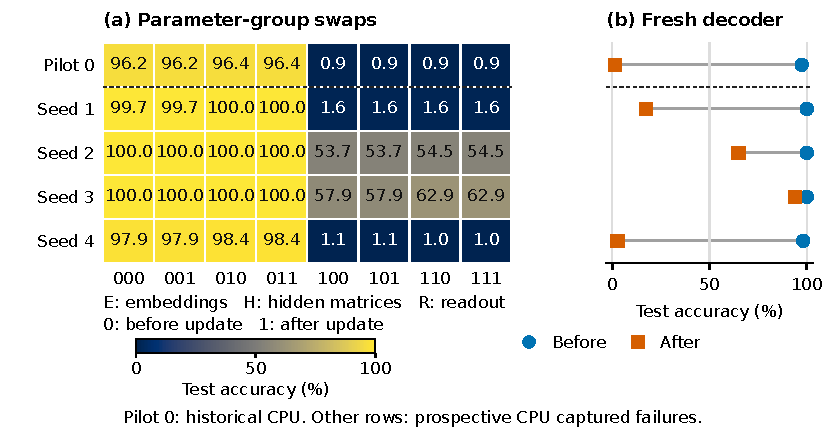
\includegraphics[width=\textwidth]{followup_rms_replication.pdf}
\caption{Accurate-CE RMS failures, with the historical pilot separated from four prospective seeds. \textbf{Left:} held-out accuracy for all eight old/new parameter-group combinations; mask order is embeddings, hidden matrices, readout. $0$ denotes the preceding state and $1$ the following state. Every updated-embedding combination gives a joint failure, while old-embedding combinations retain high accuracy. \textbf{Right:} fresh training-only decoder accuracy immediately before and after each update, using features after final RMS. All selected refits converge. Exact counts, losses, and sensitivity fits are recorded separately.}
\label{fig:rms-replication}
\end{figure}

At each prospective event, replacing only embeddings is sufficient for joint failure. With old embeddings, every combination of hidden matrices and readout retains at least $97.87\%$ test accuracy. The hidden update partly offsets the embedding damage in seeds $2$ and $3$: embeddings-only accuracy is $53.73\%$ and $57.93\%$, while applying both embedding and hidden updates gives $54.55\%$ and $62.86\%$. Readout replacement changes test accuracy by at most $0.06$ percentage points across these paired combinations. The embedding update therefore supplies the acute damage at all four captured transitions, with smaller interactions from the other groups.

All selected decoder refits before and after the five analyzed events converge. In the prospective cohort, decoder accuracy falls from $98.15$--$100\%$ before the update to $2.65$--$93.82\%$ afterward. Seed $3$ retains substantial accessibility, whereas seeds $1$ and $4$ have much lower recovery. Thus the RMS events establish an architectural boundary for both the readout locus and the uniformly high failed-state decoder recovery in the unnormalized cohort. They leave the upstream cause of the embedding displacement unresolved. Tables~\ref{tab:rms-decoder-diagnostics} and~\ref{tab:rms-derivatives} retain convergence and derivative diagnostics; full solver records and arrays accompany the paper.

Each prospective run has one sampled post-confirmation test evaluation below $95\%$, its terminal joint failure. Including confirmation, the four runs have $37$, $33$, $44$, and $27$ post-confirmation test evaluations. Their minimum sampled test accuracies equal their terminal accuracies: $1.63\%$, $54.55\%$, $62.86\%$, and $1.03\%$. These event-stopped summaries have different horizons from the pilot's subsequent recovery and from the $100{,}000$-step unnormalized continuations.

\begin{table}[htbp]
\centering\small
\setlength{\tabcolsep}{4pt}
\caption{All eight parameter-group swaps at captured RMS failures. Seed $0$ is the historical pilot; seeds $1$--$4$ are prospective. Mask order is embeddings, hidden matrices, readout; $0$ retains the preceding state and $1$ uses the following state. Accuracy is in percent. CE is accurate float64 evaluation of the resulting float32 logits. Raw records additionally retain exact counts and float32 accurate CE.}
\label{tab:rms-swaps-1}
\begin{tabular}{lrrrrr}
\toprule
Seed & EHR & Train & Test & Train CE & Test CE \\
\midrule
$0$ & 000 & 95.87 & 96.21 & 0.34207 & 0.32198 \\
$0$ & 001 & 95.87 & 96.21 & 0.33814 & 0.32056 \\
$0$ & 010 & 96.50 & 96.41 & 0.13595 & 0.20983 \\
$0$ & 011 & 96.55 & 96.41 & 0.13393 & 0.2092 \\
$0$ & 100 & 1.15 & 0.94 & 6.7289 & 6.7765 \\
$0$ & 101 & 1.12 & 0.93 & 6.7313 & 6.7788 \\
$0$ & 110 & 1.20 & 0.89 & 6.808 & 6.8589 \\
$0$ & 111 & 1.17 & 0.88 & 6.811 & 6.8617 \\
\addlinespace
$1$ & 000 & 99.53 & 99.70 & 0.0091396 & 0.0054243 \\
$1$ & 001 & 99.53 & 99.71 & 0.008633 & 0.0051797 \\
$1$ & 010 & 100.00 & 100.00 & 2.9798e-05 & 3.6247e-05 \\
$1$ & 011 & 100.00 & 100.00 & 2.945e-05 & 3.5891e-05 \\
$1$ & 100 & 1.10 & 1.61 & 5.8687 & 5.8818 \\
$1$ & 101 & 1.10 & 1.61 & 5.8695 & 5.8827 \\
$1$ & 110 & 1.07 & 1.63 & 5.8567 & 5.8698 \\
$1$ & 111 & 1.07 & 1.63 & 5.8575 & 5.8707 \\
\addlinespace
$2$ & 000 & 100.00 & 100.00 & 6.4328e-05 & 5.5268e-05 \\
$2$ & 001 & 100.00 & 100.00 & 6.324e-05 & 5.477e-05 \\
$2$ & 010 & 100.00 & 100.00 & 2.8588e-05 & 3.2462e-05 \\
$2$ & 011 & 100.00 & 100.00 & 2.857e-05 & 3.2467e-05 \\
$2$ & 100 & 54.57 & 53.73 & 3.1082 & 3.105 \\
$2$ & 101 & 54.57 & 53.73 & 3.1082 & 3.105 \\
$2$ & 110 & 55.22 & 54.55 & 3.0872 & 3.0822 \\
$2$ & 111 & 55.22 & 54.55 & 3.0872 & 3.0823 \\
\addlinespace
\bottomrule
\end{tabular}
\end{table}

\begin{table}[htbp]
\centering\small
\setlength{\tabcolsep}{4pt}
\caption{All eight parameter-group swaps at captured RMS failures. Seed $0$ is the historical pilot; seeds $1$--$4$ are prospective. Mask order is embeddings, hidden matrices, readout; $0$ retains the preceding state and $1$ uses the following state. Accuracy is in percent. CE is accurate float64 evaluation of the resulting float32 logits. Raw records additionally retain exact counts and float32 accurate CE.}
\label{tab:rms-swaps-2}
\begin{tabular}{lrrrrr}
\toprule
Seed & EHR & Train & Test & Train CE & Test CE \\
\midrule
$3$ & 000 & 100.00 & 100.00 & 0.00091077 & 0.0010679 \\
$3$ & 001 & 100.00 & 100.00 & 0.00090878 & 0.0010657 \\
$3$ & 010 & 100.00 & 100.00 & 0.00026494 & 0.00030755 \\
$3$ & 011 & 100.00 & 100.00 & 0.00026434 & 0.00030686 \\
$3$ & 100 & 58.96 & 57.93 & 2.0143 & 2.1057 \\
$3$ & 101 & 58.96 & 57.93 & 2.014 & 2.1054 \\
$3$ & 110 & 64.15 & 62.86 & 1.8055 & 1.8808 \\
$3$ & 111 & 64.15 & 62.86 & 1.8052 & 1.8805 \\
\addlinespace
$4$ & 000 & 97.65 & 97.87 & 0.14149 & 0.12772 \\
$4$ & 001 & 97.65 & 97.87 & 0.13947 & 0.12727 \\
$4$ & 010 & 99.37 & 98.36 & 0.04257 & 0.083994 \\
$4$ & 011 & 99.40 & 98.41 & 0.041476 & 0.083846 \\
$4$ & 100 & 0.84 & 1.05 & 6.3598 & 6.3671 \\
$4$ & 101 & 0.84 & 1.05 & 6.3556 & 6.3626 \\
$4$ & 110 & 0.89 & 1.03 & 6.3563 & 6.3669 \\
$4$ & 111 & 0.89 & 1.03 & 6.3517 & 6.3621 \\
\addlinespace
\bottomrule
\end{tabular}
\end{table}

\begin{table}[htbp]
\centering\small
\setlength{\tabcolsep}{4pt}
\caption{Accurate-CE derivative diagnostics on identical stored float32 training logits. Seed $0$ is the historical pilot; seeds $1$--$4$ are prospective. Errors compare the full mean-loss derivative with the analytic float64 reference. Class-sum residual is the $L_2$ norm across examples of the sum over classes. Maximum absolute errors and reference class-sum residuals are retained in the supporting records.}
\label{tab:rms-derivatives}
\begin{tabular}{llrrrr}
\toprule
Seed & State & Relative error & Absolute error & Reference norm & Class-sum residual \\
\midrule
$0$ & Before & $9.48\times10^{-8}$ & $4.06\times10^{-10}$ & $4.28\times10^{-3}$ & $4.30\times10^{-10}$ \\
$0$ & After & $5.08\times10^{-8}$ & $8.83\times10^{-10}$ & $1.74\times10^{-2}$ & $1.55\times10^{-9}$ \\
$1$ & Before & $8.12\times10^{-8}$ & $1.00\times10^{-10}$ & $1.24\times10^{-3}$ & $1.18\times10^{-10}$ \\
$1$ & After & $3.88\times10^{-8}$ & $6.35\times10^{-10}$ & $1.63\times10^{-2}$ & $1.45\times10^{-9}$ \\
$2$ & Before & $4.76\times10^{-8}$ & $1.21\times10^{-12}$ & $2.54\times10^{-5}$ & $3.67\times10^{-13}$ \\
$2$ & After & $4.86\times10^{-8}$ & $6.02\times10^{-10}$ & $1.24\times10^{-2}$ & $9.58\times10^{-10}$ \\
$3$ & Before & $8.99\times10^{-8}$ & $1.92\times10^{-12}$ & $2.13\times10^{-5}$ & $9.97\times10^{-13}$ \\
$3$ & After & $5.04\times10^{-8}$ & $5.98\times10^{-10}$ & $1.19\times10^{-2}$ & $8.80\times10^{-10}$ \\
$4$ & Before & $5.28\times10^{-8}$ & $1.40\times10^{-10}$ & $2.64\times10^{-3}$ & $2.36\times10^{-10}$ \\
$4$ & After & $4.26\times10^{-8}$ & $7.16\times10^{-10}$ & $1.68\times10^{-2}$ & $1.37\times10^{-9}$ \\
\bottomrule
\end{tabular}
\end{table}

\begin{table}[htbp]
\centering\small
\setlength{\tabcolsep}{4pt}
\caption{RMS decoder convergence and unregularized sensitivity. Seed $0$ is the historical pilot; seeds $1$--$4$ are prospective. Candidate convergence reports successful validation-candidate fits out of five; selected-refit convergence is in Table~\ref{tab:rms-event-decoders}. Unregularized accuracy is held-out percent. Complete termination messages, objectives, iteration counts, and gradient norms accompany every fit.}
\label{tab:rms-decoder-diagnostics}
\begin{tabular}{llrrrl}
\toprule
Seed & State & Selected $\lambda$ & Candidates & Unreg.\ test & Unreg.\ converged \\
\midrule
$0$ & Before & $1.00\times10^{-4}$ & 5/5 & 95.83 & Yes \\
$0$ & After & $1.00\times10^{-2}$ & 3/5 & 2.62 & No \\
$1$ & Before & $1.00\times10^{-8}$ & 5/5 & 100.00 & Yes \\
$1$ & After & $1.00\times10^{-2}$ & 5/5 & 11.05 & Yes \\
$2$ & Before & $0$ & 5/5 & 100.00 & Yes \\
$2$ & After & $1.00\times10^{-2}$ & 5/5 & 55.35 & Yes \\
$3$ & Before & $0$ & 5/5 & 100.00 & Yes \\
$3$ & After & $1.00\times10^{-6}$ & 5/5 & 88.66 & Yes \\
$4$ & Before & $1.00\times10^{-4}$ & 5/5 & 96.21 & Yes \\
$4$ & After & $1.00\times10^{-2}$ & 3/5 & 4.13 & No \\
\bottomrule
\end{tabular}
\end{table}

